\section{Gestenerkennung mit Entscheidungsbäumen}
\label{sec:sota_misc}
Song et al. \cite{song2019design} haben die Handgestenerkennung mit Gradient Boosting Entscheidungsbäumen (GBDT) untersucht. Gradient Boosting definiert boosting als numerisches Optimierungsproblem,
indem eine Kostenfunktion minimiert wird durch die iterative Summierung von schwachen Lernern, die durch den Gradient Descent Algorithmus gefunden wird \cite{friedman1999greedy}. Sie wählten einen nicht-optischen
Ansatz, der mit Hilfe eines tragbaren sEMG Recorders die elektrischen Signale der Muskelaktivitäten erfasst. Als Eingabe für den Entscheidungsbaum wählten sie neun Features (siehe Tabelle \ref{tab:songFeatures}).
Damit erzielten sie eine Klassifizierungsgenauigkeit von 91\% unter zwölf verschiedenen Handgesten.
\begin{table}[h!]
    \centering
    \begin{tabular}{ | c | c | c | }
        \hline
        1 & Mean absolute value & $\frac{1}{N}\sum^N_{t=1} |x_t|$ \\\hline
        2 & Simple square integral & $\sum^N_{t=1} |x_t|^2$ \\\hline
        3 & Minimum value & $\min x_t$ \\\hline
        4 & Maximum value & $\max x_t$ \\\hline
        5 & Standard deviation & $\sqrt{\frac{1}{N}\sum^N_{t=1}(x_t - \tilde{x})^2}$ \\\hline
        6 & Average amplitude change & $\frac{1}{N-1}\sum^{N-1}_{t=1} |x_{t + 1} - x_t|$ \\\hline
        7 & Zero crossing & $\sum^{N-1}_{t=1}diff(sgn(x_{t+1}),sgn(x_t))$ \\\hline
        8 & Slope sign change & $\sum^{N-2}_{t=1}diff(sgn(x_{t+1} - x_t),sgn(x_t - x_{t - 1}))$ \\\hline
        9 & Willison amplitude & $\sum^{N-1}_{t=1}u(|x_{t+1} - x_t| - threshold)$ \\
        \hline
    \end{tabular}
    \caption{Die von Song et al. genutzten Features \cite{song2019design}.}
    \label{tab:songFeatures}
\end{table}
\newline
\newline
Ahad et al. \cite{ahad2012motion} diskutieren den Motion History Image (MHI) Ansatz. MHI ist ein optischer Ansatz, der eine Sequenz von Bildern in ein einziges Bild komprimiert. Dabei werden Bewegungen,
die nach anderen Bewegungen stattgefunden haben heller angezeigt. Die Funktion $\psi(x,y,t)$ bestimmt, ob eine Bewegung in einem Pixel $(x,y)$ zu einem Zeitpunkt $t$ stattfindet.
\newline
\newline
Formel \ref{formular:mhi} beschreibt die rekursive Berechnung des MHI. Das MHI kann aber auch sequenziell berechnet werden. Initial sind alle Werte 0. Wenn $\psi(x,y,t)$ eine Bewegung in einem Pixel $(x,y)$
zu einem Zeitpunkt $t$ signalisiert, dann wird der Pixel auf den Maximalwert $\tau$ gesetzt. Mit jedem Bild, indem keine Bewegung im Pixel $(x,y)$ durch $\psi$ signalisiert wurde, wird der Wert um den
Zerfallswert $\delta$ dekrementiert bis zu einem Minimum von 0.
\begin{align}
    H_{\tau}(x,y,t) = \begin{cases}
                          \tau & if \psi(x,y,t) = 1 \\
                          \max(0, H_{\tau}(x,y,t-1) - \delta) & otherwise
    \end{cases}
    \label{formular:mhi}
\end{align}
MHI ist leicht zu berechnen und invariant zu Lichtverhältnissen. Allerdings ist die Leistung stark abhängig von $\psi$, $\tau$ und $\delta$. MHI ist besonders anfällig für Bildfolgen mit verschiedener Länge.
Je nachdem, wie $\tau$ und $\delta$ gewählt sind, ist die Bewegungshistorie nicht sichtbar oder der Einfluss der ersten Bilder geht verloren.
\newline
\newline
Abbildung \ref{fig:mhi_ex} zeigt ein Motion History Image einer Bildsequenz. In der Bildsequenz wird eine Armbewegung ausgeführt. Unter jedem Bild ist das resultierende MHI zu dem Zeitpunkt zu sehen.
Zu sehen ist, dass Pixel die sich verändert haben weiß sind und die anderen Pixel schwarz. Mit der fortlaufenden Bildsequenz wird das Bild erweitert und der Arm scheint sich zu duplizieren und seine
Vergangenheit hinter sich her zu ziehen. Diese vergangene Bewegung ist aber dunkler als die kürzlich ausgeführten Bewegungen. Dies wird als die Historie des MHI bezeichnet. Durch den Zerfallswert sind
vergangene Bewegungen dunkler.
\begin{figure}
    \centering
    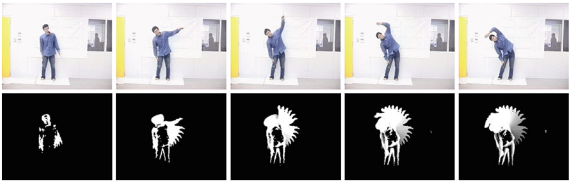
\includegraphics[width=\linewidth]{images/mhi_ex.png}
    \caption{Die Übersetzung von einer Bildsequenz zu einem Motion History Image. Übernommen aus der Arbeit von Ahad et al. \cite{ahad2012motion}.}
    \label{fig:mhi_ex}
\end{figure}